\documentclass[12pt,letterpaper]{article}
\usepackage{amsmath}
\usepackage{amsfonts}
%\usepackage{color}
\usepackage[usenames,dvipsnames]{color}
\usepackage{graphicx}
\usepackage{longtable}
\usepackage{rotating}
\usepackage{verbatim}
\usepackage[pdftex,bookmarksopen]{hyperref}
\hypersetup{pdfauthor={John Sibert}}
\hypersetup{pdfsubject={Compartment model of MHI YFT}}
\hypersetup{pdftitle={Two-compartment models of Main Hawaiian Islands
Yellowfin Tuna Population}}
\hypersetup{pdfkeywords={yellowfin,state space,compartment model,Hawaii}}

\newcommand\doublespacing{\baselineskip=1.6\normalbaselineskip}
\newcommand\singlespacing{\baselineskip=1.0\normalbaselineskip}
\renewcommand\deg[1]{$^\circ$#1}
\newcommand\SD{SEAPODYM}
\newcommand\MFCL{MULTIFAN-CL}
\newcommand\ADMB{ADModel Builder}
\newcommand\SPC{Secretariat of the Pacific Community}
\newcommand\WCPO{Western Central Pacific Ocean}
\newcommand\SSAP{Skipjack Survey and Assessment Programme}
\newcommand\RTTP{Regional Tuna Tagging Programme}
\newcommand\PTTP{Pacific Tuna Tagging Programme}
\newcommand\FAD{fish aggregating device}
\newcommand\ADRM{advection-diffusion-reaction model}
\newcommand\help[1]{\color{Magenta}{\it #1 }\normalcolor}
\newcommand\widebar[1]{\overline{#1}}
\newcommand\EEZ{Exclusive Economic Zone}

\newcommand\None{{N_{1,1}}}
\newcommand\Ntwo{{N_{2,1}}}
\newcommand\Nsum{{N_{1,1}+N_{2,1}}}
\newcommand\peryr{yr$^{-1}$}
\newcommand\prevN[1]{{#1_{t-\Delta t}}}
\newcommand\nextN[1]{{#1_t}}

\title{Compartment models of Main Hawaiian Islands Yellowfin Tuna
Populations\\
~\\
Interim Report}

\author{
John Sibert\thanks{sibert@hawaii.edu}\\
Joint Institute of Marine and Atmospheric Research\\
University of Hawai'i at Manoa\\
Honolulu, HI  96822 U.S.A.\\[0.125in]
\date{\today}
}

\pagestyle{myheadings}
\markright{Sibert\hfil {\bf INTERIM} MHI Comparment Model\hfil\today}

\begin{document}
\maketitle

\doublespacing

\section*{Introduction}
The Yellowfin Tuna (YFT) population in main Hawaiian Islands (MHI) is
embedded in a larger pan-Pacific stock. Nevertheless, local fishermen
believe that the MHI supports a ``resident'' yellowfin population.
Some scientific observations are consistent with this belief. 
Recent tagging and tracking
studies show that the rate of exchange between the MHI population
and the larger stock is low (Itano and Holland 2000). Analysis
of YFT otoliths sampled from
throughout the Pacific conclude that 90\% or more of the MHI
population was reared in the MHI (Wells et al 2012).
The average annual catch of YFT in the MHI from 2008 through 2012 by Hawaii
based fleets was approximately 814 mt. 
Although the MHI fishery is quite small and embedded in a much larger
stock, management of this
fishery is an important local issue deserving of scientific support.

This paper explores potential models that might be used to
inform development of options for the management of fisheries for YFT
in the MHI.

The principle assumptions for modeling the MHI YFT population are:
\begin{enumerate}
\item The Pacific Ocean near Hawaii is divided into two regions:
MHI (region 1) and elsewhere (region 2).%; see Figure~\ref{fig:MHImap}.
\item Fish emigrate from region 1 to region 2, but emigrant fish have
no effect on region 2 population dynamics, i.e., region 2 is an ``infinite
sink''.
\item Fish immigrate from region 2 to region 1, and mix completely.
\item Immigrant fish are indistinguishable from ``resident'' fish
(i.e., both groups of fish have the same population dynamics) and
interact with the fishing gear in region 1 identically.
\item Immigration into the MHI is dependent on the
biomass of the yellowfin population outside of the MHI as estimated by
some other model, e.g., \MFCL\ (MFCL) or \SD.
\item The fishery comprises several gear types, each characterized by 
a distinct fishing mortality.
\item The evolution of fishing mortality over time is a random walk,
i.e., the fishing mortality in the current time step is equal
to the fishing mortality in the previous time step plus a random
deviation.
\end{enumerate}

\section*{Data}
Several sources of data are used in this analysis:
\begin{enumerate}
\item  Yellowfin catch weights reported to the Hawaii Department of Aquatic
Resources (HDAR) from 1949 to 2014.
\item Longline yellowfin catch weights reported to the National Oceanic and
Atmospheric Administration, National Marine Fisheries Service (NOAA)
under the federally mandated log book program from 1995 through 2013.
\item Measurements of average yellowfin fish weights sampled at the
Honolulu auction by NMFS staff from 2000 through 2013.
\item Model estimates of yellowfin biomass by MFCL
from the most recent WCPFC stock assessment (Davies et al 2014).
\end{enumerate}
All data are reported by quarter of the year.

\subsection*{Catch Time Series}
%The Hawaii longline fishery has a long history and changed radically
%in the 1990s when new vessels entered the fleet and fishing gear was
%modernized.
%The HDAR longline data covers the period 1949 through 2001 and does
%not differentiate between ``deep'' and ``shallow'' sets.
%The NOAA longline data covers the period 1995 through 2013 and reports deep
%and shallow set set separately.
%Thus the period of most radical change is included in time series.

%[1] Aku boat          Bottom/inshore HL Longline          Other            
%[5] Troll             Tuna HL           Casting           Hybrid           
%[9] Shortline         Vertical line    

% statistics of catch time series first differences
%TS                 Mean     S. D.
%OffshoreHL  0.017659002 0.5994987
%Troll       0.018124404 0.7051216
%Longline    0.002425213 0.7782023
%InshoreHL  -0.002342312 0.6935796
%AkuBoat    -0.004970204 1.0908600



The HDAR data comprise catch reports for the following gear
categories:
``Aku boat'', ``Bottom/inshore HL'', ``Longline'',  ``Troll'', ``Tuna
HL'', ``Casting'', ``Hybrid'',  ``Shortline'', ``Other'', and
``Vertical line''.
For this analysis catches by ``Casting'', ``Hybrid'',
``Shortline'', ``Other'', and ``Vertical line'' are combined into a new
category, ``Misc.''. The ``Misc''
catches are highest after year 2000,
but comprise a very small proportion of the catch.
The ``Aku Boat'' fishery was a small pole and line fishery
targeting skipjack tuna in Hawaii, for which yellowfin is an
incidental catch. 
The catch time series for the HDAR data are shown in
Figure~\ref{fig:hdarTS}. These time
series exhibit marked annual cycles suggesting a strong seasonal
signal in the catches by all gears.
Some series also contain sustained periods of zero catch which
document the development and subsequent shift away from a specific
gear type. It is assumed that these declines in catches represent a
``collapse'' of a fishery due more to social and economic factors than
to a decline of stock.
Some time series are punctuated by brief episodes (one or two quarters in
length) of zero catches. Again it is assumed that these zero catches
are not caused by low stock levels.

The longline fishery has changed drastically over time. In the late
1940s, it was a relatively small fishery using traditional
Okinwawan-style gear \help{(reference)}, usually labeled ``flag
line''. Participation in this fishery generally declined from 1950 to
late 1980s, as can be seen in the time series plots. In the 1990s, the longline
fishery expanded rapidly with the introduction of US fishing boats
from the Atlantic ocean using modern monofilament longline gear and
deeper sets.

Figure~\ref{fig:hdarTS} also displays the first order differences
between successive quarters. This statistic emphasizes the seasonal
periodicity of all fishing gears and helps to identify potential anomalies in
the data such as changes in reporting protocols. 

The partial autocorrelations within each time
series are shown in Figure~\ref{fig:catchPACF}. These correlations
confirm the quarterly periodicity  of the catch time series.
The catch time series for Inshore HL,Longline, Troll, and Tuna HL show
similar patters with
significant positive autocorrelations at lags of 1,3 and 4 quarters.
The autocorrelation pattern appears to be somewhat different for the Aku
boat catch time series.

NOAA began to collect data from the longline fleet under a federally
mandated logbook program in 1990, and in 1995, began to distinguish
deep and shallow setting in the data. The HDAR data do not
distinguish between deep and shallow sets.
Figure~\ref{fig:hdarnoaaLLTS} shows the correspondence between the
HDAR and NOAA time series. The combined deep plus shallow catches from
NOAA line up fairly well with the overlapping HDAR data. The simple
average of the HDAR data with the combined NOAA deep plus shallow data
appears to have roughly the same autocorrelation structure as the
constituent time series, Figure~\ref{fig:LLpartialacf}.
\help{Data are also available from NOAA for the period 1990-1995, but
have not yet been included in this analysis.}


\begin{figure}
\begin{center}
\includegraphics[height=0.8\textheight]{./graphics/hdar_catch_history.pdf}
\caption{\label{fig:hdarTS}
Yellowfin catch in metric tonnes by principle fisheries operating in
the Main Hawaiian Islands from the HDAR data.
The dotted red line superimposed on each time series is the difference in
catch between successive quarters.
The red tick marks on the abscissa indicate quarters where catches
were zero.
}
\end{center}
\end{figure}

\begin{figure}
\begin{center}
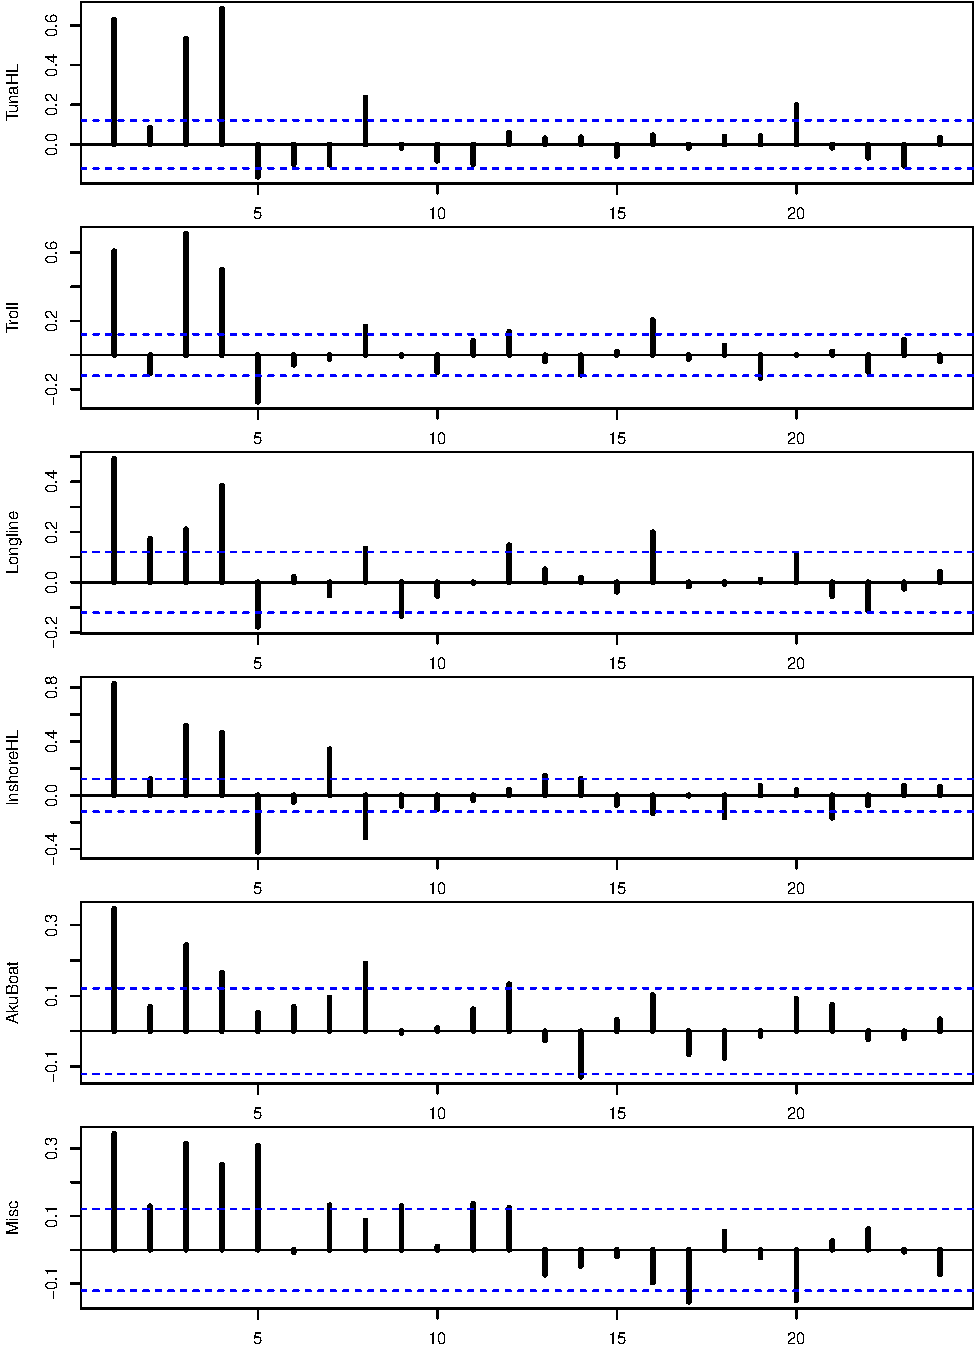
\includegraphics[height=0.8\textheight]{./graphics/partial_acf.pdf}
\caption{\label{fig:catchPACF}
Partial autocorrelation coefficients of the catch time series. The
dashed blue lines indicate approximate 95\% confidence limits of the
correlations.}
\end{center}
\end{figure}

\begin{figure}
\begin{center}
\includegraphics[height=0.8\textheight]{./graphics/hdar_noaa_LL_ts.pdf}
\caption{\label{fig:hdarnoaaLLTS}
Comparison between HDAR and NOAA longline time series. The upper panel
shows the NOAA deep and shallow set data superimposed on the HDAR
data. The lower panel shows the time series produced by a simple
average of the HDAR data and the sum of the NOAA deep and shallow
catches.}
\end{center}
\end{figure}

\begin{figure}
\begin{center}
\includegraphics[height=0.8\textheight]{./graphics/LL_partial_acf.pdf}
\caption{\label{fig:LLpartialacf}
Partial autocorrelations within the NOAA and combined time
series. F refers to the HDAR longline data, D refers to the NOAA deep
set data, S to the shallow set data,
DS to the combined deep and shallow set data, and Mean to the average
of the HDAR and NOAA deep plus shallow.
}
\end{center}
\end{figure}

\begin{figure}
\begin{center}
\includegraphics[height=0.8\textheight]{./graphics/first_difference_histograms.pdf}
\caption{\label{fig:diff1histo}
Histograms of first differences of the logarithm of catch time series. 
The blue line is
a normal distribution with the same mean and standard deviation as the
first differences. The red line is the equivalent t-distribution.}
\end{center}
\end{figure}

\begin{figure}
\begin{center}
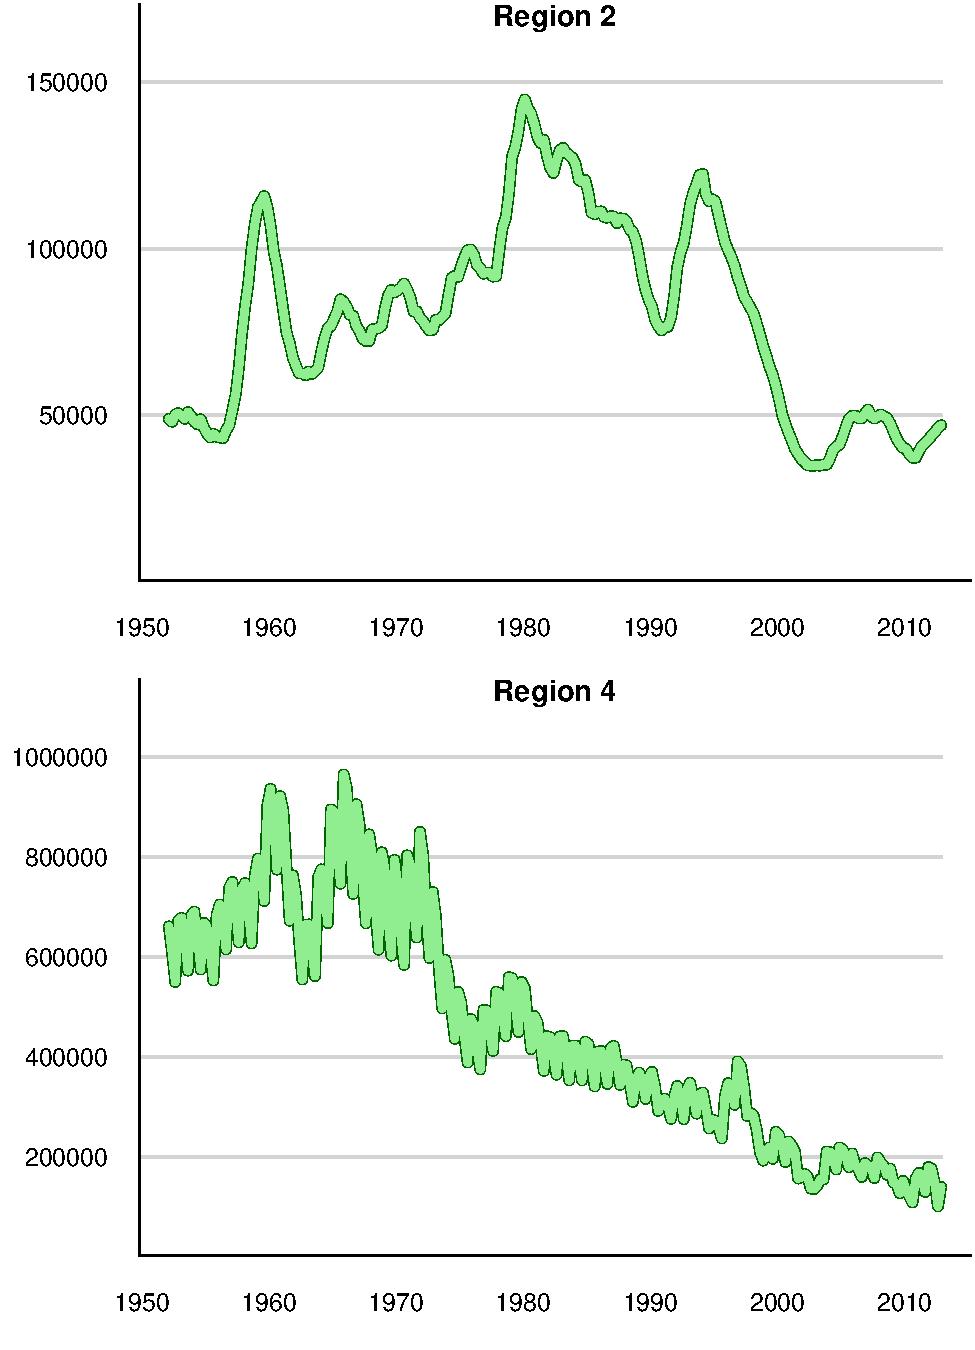
\includegraphics[height=0.8\textheight]{./graphics/MFCL_region_biomass.pdf}
\caption{\label{fig:MFCLregionB}
Estimates of biomass in MFCL Regions 2 and 4 from the 2104 WCPFC YFT
stock assessment, Davies et al. 2014. The green lines are the biomass
trends. Dotted red and blue lines are first and second differences
respectively.}
\end{center}
\end{figure}

%\begin{figure}
%\begin{center}
%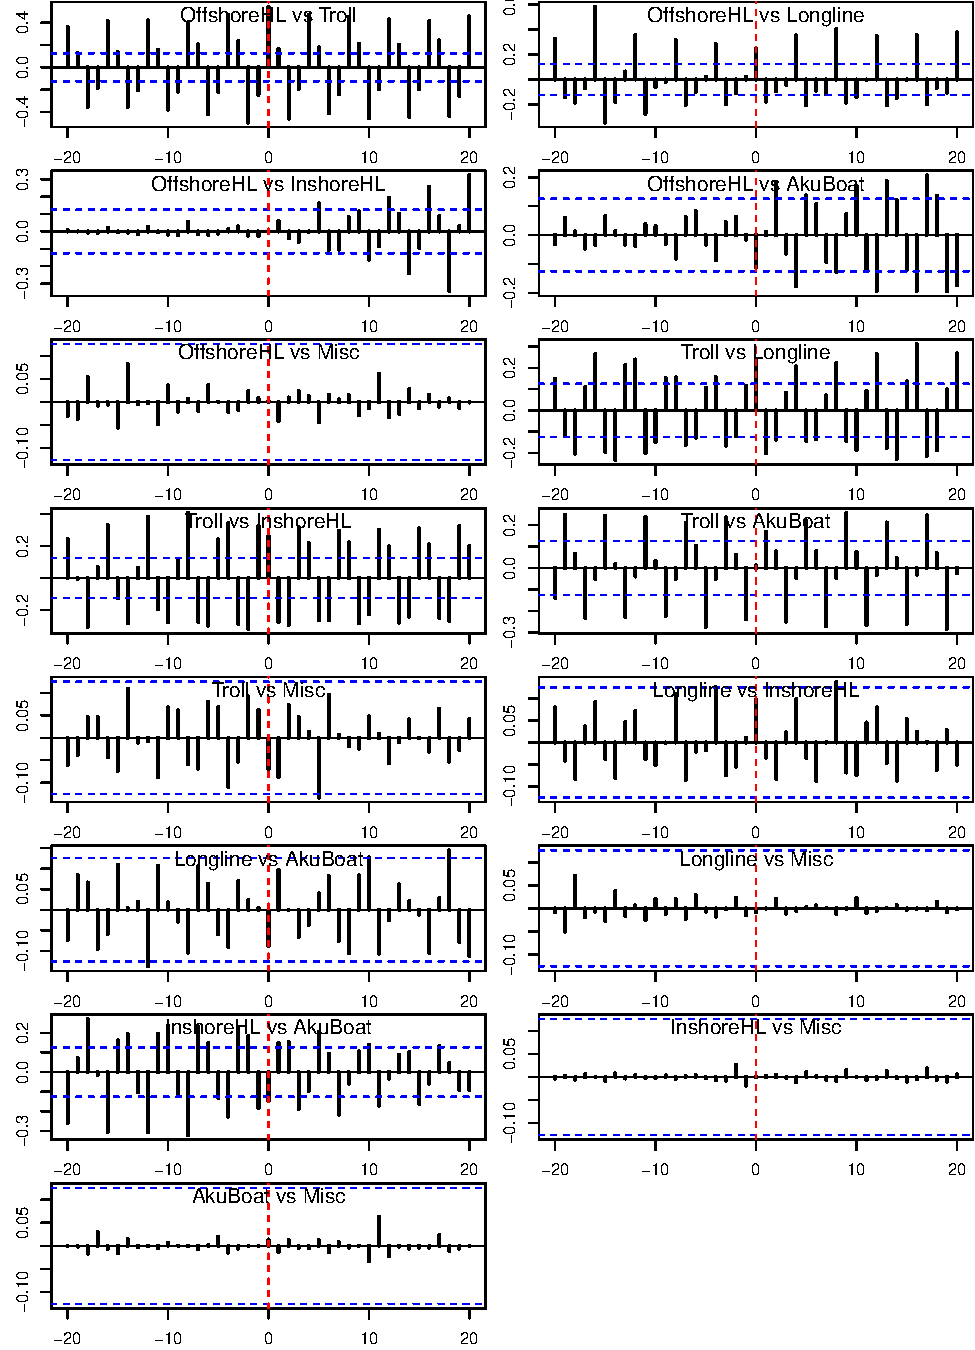
\includegraphics[height=0.8\textheight]{./graphics/ccf.pdf}
%\caption{\label{fig:catchCCF}
%Cross correlation coefficients between pairs of the first order
%differences of each catch time series at different lags.
%The vertical dashed red line emphasize zero lag.
%The dashed blue lines indicate approximate 95\% confidence limits of
%the correlation coefficients.}
%\end{center}
%\end{figure}

\subsection*{Fish Weight Time Series}
~
\centerline{\help{Not yet available.}}

%\clearpage
\section*{Models}
The general modeling approach is to develop a state-space model
similar to that utilized by Nielsen and Berg (2014).
State-space models separate variability in the biological
processes in the system (transition model)
from errors in observing features of interest
in the system (observation model). 
The general form of the transition equation is
\begin{equation}
\alpha_t=T(\alpha_{t-1}) + \eta_t
\end{equation}
where the function $T$ embodies the stock dynamics mediating the
development of the state at time $t$ from the state at the previous
time with random process error, $\eta$.
The general form of the observation equation is
\begin{equation}
x_t = O(\alpha_t) + \varepsilon_t
\end{equation}
where the function $O$ describes the measurement process and with
error $\varepsilon$

\subsection*{Age-aggregated model: logistic population dynamics}

Let $\None$ equal the biomass of fish originating in region 1
and residing in region 1
and $\Ntwo$ equal the biomass of fish originating in region 2
but residing in region 1.
The total biomass of fish residing in region 1 is
$\Nsum$, and the dynamics of the population in region 1 is represented
as a modified Schaefer Model:
\begin{equation}
\frac{d}{dt}\big(\Nsum\big)=\big(\Nsum\big)\Big[r\Big(1-\frac{\Nsum}{K}\Big)-F-T_{12}\Big]+T_{21}
\label{eqn:logistic}
\end{equation}
where $r$ is the logistic growth rate per quarter, $K$ is the
asymptotic biomass,
$F$ is the total fishing mortality in region 1, $T_{12}$
is the emigration rate from region 1 to region 2, and $T_{21}$
is the annual rate of immigration of biomass from region~2 to region~1.


An equivalent differential equation could be devised for the dynamics of
fish residing in region 2 
(i.e., $\frac{d}{dt}\big(N_{2,2}+N_{1,2}\big)$), but 
the dynamics of the fish population in region 2 is external to this
model. $T_{21}$ can be considered to be form of population ``forcing''
by the larger stock in which the MHI population is embedded. $T_{21}$
could a prediction from other models, such as \MFCL\ or \SD, in a sort of
``off-line'' coupling, or perhaps represented by an
autocorrelated stochastic process. 

The appearance of
$\Nsum$ in the numerator of the logistic term reflects the assumption
that the population dynamics of immigrant fish depends on
the population dynamics in region 1. This assumption leads to an
important non-linearity in the model that predicts the possibility of
overwhelming of the
local stock by a more numerous immigrant stock as is often characteristic of
mixed-stock fisheries.

The proportion of ``local'' fish $\frac{\None}{\Nsum}$ is of potential interest.
Equation~\ref{eqn:logistic} can be expanded and rearranged to become
\begin{eqnarray}
\label{eqn:coupledschaefer}
\frac{d}{dt}\big(\Nsum\big) &=&\None\Big[r\Big(1-\frac{\None}{K}\Big)
-F - T_{12}\Big] \nonumber\\
&+&\Ntwo\Big[r\Big(1-\frac{\Ntwo}{K}\Big)
-F - T_{12}\Big]  + T_{21}\\
&-& 2r\frac{\None\Ntwo}{K}\nonumber
\end{eqnarray}
The non-linear term, $2r\frac{\None\Ntwo}{K}$, in
equation~\ref{eqn:coupledschaefer} represents the reduction in biomass
of one population by the presence of the other population.
In order to represent
the two populations by separate equations, this
nonlinear term must be appropriately apportioned.
A new parameter, $q$, is introduced to accomplish the apportionment,
leading to a set of simultaneous non-linear differential equation for the
components of the population inhabiting region~1.
\begin{eqnarray}
\label{eqn:coupledschaeferq}
\frac{d\None}{dt}&=&\None\Big[r\Big(1-\frac{\None}{K}\Big)
-F - T_{12}\Big] - (1-q)2r\frac{\None\Ntwo}{K}\nonumber\\
\\
\frac{d\Ntwo}{dt}&=&\Ntwo\Big[r\Big(1-\frac{\Ntwo}{K}\Big)
-F - T_{12}\Big] - q2r\frac{\None\Ntwo}{K} + T_{21}\nonumber
\end{eqnarray}
\help{Does this system have a meaningful equilibrium with both
$\None > 0$ and $\Ntwo > 0$?}

%The equilibrium of this system can be found by setting
%$\frac{d\None}{dt} = 0 = \frac{d\Ntwo}{dt}$. After some simplification
%the result is $\frac{T_{21}}{\Ntwo} = 0$. In other words, there is no
%equilibrium in this coupled system, other than the degenerate case of
%no immigration ($T_{21}=0$) into the region 1. Thus, the notion of using
%equilibrium-based reference points such as MSY to manage fisheries for
%MHI yellowfin is ill advised.

The log transformed equivalent of equation~\ref{eqn:coupledschaeferq}
is
\begin{eqnarray}
\label{eqn:coupledlogschaefer}
\frac{d\log(\None)}{dt}&=&r\Big(1-\frac{\None}{K}\Big) -F - T_{12} -
(1-q)2r\frac{\Ntwo}{K}\nonumber\\
\\
\frac{d\log(\Ntwo)}{dt}&=&r\Big(1-\frac{\Ntwo}{K}\Big) -F - T_{12} -
q2r\frac{\None}{K} + \frac{T_{21}}{\Ntwo}\nonumber
\end{eqnarray}

{\bf Transition Equation $T(\alpha_{t-1})$.}
The state space transition equation for the two components of the MHI
population is developed by solving
equations \ref{eqn:coupledlogschaefer} by finite differences
with explicit time stepping and adding process error
terms.
\begin{eqnarray}
\log \None_t &=& \log \None_{t-\Delta t}\nonumber\\ 
             &+&\Delta t\bigg(r\Big(1-\frac{\None_{t-\Delta t}}{K}\Big)
-\sum_{g=1}^n F_{g,t-\Delta t} - T_{12} - (1-q)2r\frac{\Ntwo_{t-\Delta
t}}{K}\bigg)+\eta_{1,t}\nonumber\\
\\ \log \Ntwo_t &=& \log \Ntwo_{t-\Delta t}\nonumber\\
             &+&\Delta t\bigg(r\Big(1-\frac{\Ntwo_{t-\Delta t}}{K}\Big)
-\sum_{g=1}^n F_{t-\Delta t} - T_{12} - q2r\frac{\None_{t-\Delta t}}{K}
     +\frac{T_{{21}_{t-\Delta t}}}{\Ntwo_{t-\Delta t}}\bigg)+\eta_{2,t}\nonumber
\label{eqn:finitecoupledlogschaefer}
\end{eqnarray}
where $\eta_{k,t} \sim N(0,\Sigma_\eta),k=1,2$. The covariance matrix,
$\Sigma_\eta = \left[\begin{array}{cc}\sigma^2_{\eta,1}&\rho_\eta\\
                                     \rho_\eta&\sigma^2_{\eta,2}
\end{array}\right]$,
expresses process errors for both populations as well as a
correlation between the errors.

{\bf Fishing Mortality.}
Fishing mortality is
modeled explicitly as a random walk
without recourse to effort standardization or
estimation of catchability coefficients. The logarithm of fishing
mortality is assumed to
follow a random walk with normal increments, i.e.,
\begin{equation}
\log F_{g,t} = \log F_{g,t-1} + \xi_{g,t};\quad \xi_{t,g}\sim
N(0,\sigma^2_{\xi,g}) \label{eqn:Fwalk}
\end{equation}
where  $\sigma^2_{\xi,g}$ is the variance of the fishing
effort random walk for gear $g,\; g=1\ldots n$.

%Parameterization of $T_{21}$
{\bf Population Forcing $T_{21}$.}
Immigration of stock from region 2 to region 1 is a
form of forcing whereby events outside of the model influence the
model dynamics. The term $T_{{21}_t}$ is the biomass immigrating
into the MHI stock at each time step. 
The likely candidates for forcing are MFCL regions 2 and 4, both of
which overlap the MHI. The estimated biomass trajectories for these
two regions are shown in Figure~\ref{fig:MFCLregionB}.
For testing purposes,
I assume that source of immigrants is MFCL region 2, so that
\begin{equation}
T_{{21}_t} = T^*_{21}\cdot B_{2,t}
\end{equation}
where $B_{2,t}$ is biomass in region 2 at time $t$ taken from the MFCL output file
{\tt plot-12.par.rep} from the 2014 WCPFC stock assessment
(Davies et al 2014). $T^*_{21}$ is the proportion on
$B_{2,t}$ which migrates at each time step.
Alternatively, $B_{2,t}$ may be assumed to be constant at the average
of the estimated biomass in region 2, $\widebar{B_{2}}$.

{\bf Parameterization of $K$.}
$K$ is the asymptotic biomass in a population growing according to
logistic dynamics. It is the population size to which the population
tends at equilibrium and is often dubbed ``carrying capacity''. 
It is not clear that a coupled logistic model such as
\ref{eqn:logistic} has a non-trivial equilibrium. Furthermore the
$B_{2,t}$ is time dependent, Figure~\ref{fig:MFCLregionB}.
Several alternative
parameterizations of $K$ can be envisaged, for example, constant at
the maximum of $B_{2,t}$, an unknown parameter, or even a random walk.
For testing purposes I have assumed the maximum of $B_{2,t}$ because
the maximum biomass is lower in region 2 and appears less depleted
than in region 4.

Given that the model forcing $B_{r,t}$ is not constant and that the
fishery is developing in a period of profound change in the oceans,
it is difficult to justify the assumption of constant $K$. An
alternative parameterization for $K$ is to assume a random walk, for
example,
\begin{equation}
\log K_t = \log K_{t-1} + \omega_t;\quad \omega_t\sim
N(0,\sigma^2_\omega) \label{eqn:Kwalk}
\end{equation}
where  $\sigma^2_\omega$ is the characteristic variance of the
asymptotic population size random walk.
This parameterization was implemented in code, but not extensively
tested.

{\bf Observation Equation, $O(\alpha)$.}
Predicted catch in region 1 is the product of fishing mortality
and the total population in region, $\None+\Ntwo$.
Thus the state-space observation model predicting catch in the region 1
under this model is
\begin{equation}
\log C_{g,t} = \log \Biggl(F_{g,t}\cdot\Bigl(\frac{\None_{t-\Delta t}+\None_t}{2}
                           +\frac{\Ntwo_{t-\Delta
t}+\Ntwo_t}{2}\Bigr)\Biggr) + \varepsilon_{t,g}
\label{eqn:obs}
\end{equation}
where the total population in region 1 is the sum of the average
population over the time step (Quinn and Deriso, 1999), and
$\varepsilon_{t,g} \sim N(0,\sigma^2_{\varepsilon,g})$.

{\bf Constraint on ``Proportion Local''.}
Proportion local is defined as $p = \frac{\None}{\Nsum}$. The logit
transformed proportion local, $L(p)$, is assumed to be normally
distributed around a mean value, $L(\bar{p})$.
\begin{equation}
\label{eqn:LpropL}
L(p)\sim N(L(\bar{p}),\sigma^2_{L(p)}).
\end{equation} 
$p$ is generally assumed to be approximately $0.9$. By varying the
value of the variance, $\sigma^2_{L(p)}$, $p$ can be made as
close to $0.9$ as is prudent.
This representation of $p$ can be interpreted as a Bayesian prior.
In principle, it may be possible to
estimate $\bar{p}$ and $\sigma^2_{L(p)}$, but interactions with
the parameter $q$ in equation~\ref{eqn:coupledschaeferq} needs to be
explored.

{\bf Estimation.} The model states, $\alpha_t$, are assumed to be random
effects (Skaug and Fournier, 2006). Model parameters are estimated by
maximizing the joint likelihood of the random
effects and the observations.
\begin{equation}
L(\theta,\alpha,x)=
\prod^m_{t=2}\big[\phi\big(\alpha_t-T(\alpha_{t-1}), \Sigma_\eta\big)\big]
\prod^m_{t=1}\big[\phi\big(x_t-O(\alpha_t), \Sigma_\varepsilon\big)\big]
\end{equation}
Here, $m$ is the number of time steps in the catch time series and
$\theta$ is a vector of model parameters. A complete list of
parameters is found in Table~\ref{tab:allvars}. 
The model is implemented in AD Model Builder (Fournier et al 2012).
The actual number of
parameters to be estimated depends on the model configuration,
specified by the phase flags in the input file. 
All computer code, data files, and draft reports in support of this
analysis can be found at Github:\linebreak
\url{https://github.com/johnrsibert/XSSA.git}.


\begin{table}
\caption{Model variables.
\label{tab:allvars}}
\begin{center}
\begin{tabular}{ll}
\hline
Variable & Definition\\
\hline
\hline
$m$ & Number of quarterly time steps\\
$n$ & Number of fishing gears\\
\hline
\hline
$r$ & Instantaneous growth rate $(q^{-1})$\\
$K$ & Asymptotic biomass (mt) \\
$T_{12}$ & Emigration rate $(q^{-1})$\\
$T^*_{21}$& Immigration rate $(q^{-1})$\\
$\sigma_{1,\eta}, \sigma_{2,\eta}$ & Population growth SD\\
$\rho_\eta$ & Correlation between population growth precess errors\\
$\sigma_{\xi,g}\; g=1\ldots n$ & Fishing mortality random walk SD\\
$\sigma_{\varepsilon,g}\; g=1\ldots n$ & Observation error SD \\
$\bar{p}$ & Mean proportion local\\
$\sigma_{L(p)}$ & SD logit transformed $p$\\
$q$ & Nonlinear apportionment proportion\\
$a_g\; g=1\ldots n$ & Proportion of $F$ random walk contaminated by 
fat-tailed distribution\\
\hline
\end{tabular}
\end{center}
\end{table}

\subsection*{Age-structured models}
~
\centerline{\help{Not yet available.}}

\section*{Results \& Discussion}
Initial model testing gives mixed results. The numerical estimation
procedure inevitably terminates with the dreaded error message 
\help{``Matrix not positive definite in Ln\_det\_choleski''.}
Values of the model parameters just prior to termination of the program are
compared to their initial values in Table~\ref{tab:testrun}.
The model seems sensitive to the population dynamics parameters. The
values of the
growth rate and transfer rates parameters ($r,T_{12}, T_{21}^*$)
change substantially from their initial values.
The state equation process errors, $\sigma_{1,\eta},\sigma_{2,\eta}$,
also move away from their initial values.
The process error correlation, $\rho$, is not yet implemented in the model
code which is equivalent to constraining $\rho$ to be zero.

The random-walk representation of fishing mortality
produces a credible time series
capable of accurately predicting catches
of all 5 gear types in the model, 
Figures~\ref{fig:estC} and~\ref{fig:estF}.
These estimates of $F$ depend on a ``robust'' likelihood representation
of the variance of the random walk with a 5\% contamination by a fat-tailed
distribution to accommodate outliers; $a_g$ in Table~\ref{tab:testrun}.

Fifteen parameters are used to represent the variance in catch, $a_g$, 
$\sigma_{\varepsilon,g}$ and $\sigma_{\xi,g}$.
These parameters are changed little or not at all by the estimation
procedure, suggesting that some are redundant.
It may be possible to represent these errors by a single parameter for
each fleet.

The predicted biomass corresponding from the test run is shown in
Figure~\ref{fig:estB}. After some fluctuations at the beginning of
the time series the total biomass, $\Nsum$, appears to stabilize to a
constant value slightly below the asymptotic biomass, $K$. The
proportion local stays close to 0.9 as it is constrained to do by the
prior, equation~\ref{eqn:LpropL}.
In other test runs (not illustrated here), 
the total biomass is less steady and has an
increasing and subsequent decreasing trend reflecting the trend in the
forcing biomass.
The cause of the initial fluctuation in
Figure~\ref{fig:estB} is unknown. The procedure seems
to set the initial population random effects higher than $K$ for some
reason.

The catch time series include a fairly large number of zero catch
observations, Figures~\ref{fig:hdarTS} and~\ref{fig:diff1histo}.
Zero observations at the
beginning of the time series, as the fishery develops, or at the end of
the time series, as a particular fleet ceases operation, do not appear
to cause problems in estimating $F$.
However, in the case of the Troll, Inshore Handline and Aku Boat
fleets, there are isolated quarters where the reported catch is zero
during periods of substantial catch.
In early test runs of the model, these observations caused the model to predict
zero biomass at those quarters followed by periods of recovery. 
The problem of intercalated zero observations
was provisionally solved by substituting the average of the immediately
preceding and following observations for the intercalated zero
observation. There are 9 such substitutions among the 1220
observations. Another approach would be to shift annual time steps,
thus averaging out the zero observations.

There appear to be excessive numbers of zero first differences
in the data for most gears, Figure~\ref{fig:diff1histo}. Only one
gear, Aku Boat, appears to have particularly fat tails. A zero
inflated distribution may be a better choice of error model for the
fishing mortality random walk than a robustified Normal.

\begin{table}
\caption{\label{tab:testrun}
Model ``estimates''. Initial values of model parameters and
final values just prior to program exit with 
``Matrix not positive definite in Ln\_det\_choleski'' message.
``---'' indicates that the variable was constrained to be constant at
its initial value, i.e., not estimated.
}
\begin{center}
\begin{tabular}{lrr}
\hline
Vatiable & Initial Value & Final Value\\
\hline
$m$ &  244\\
$n$ &  5\\
\hline
$r$ & 0.100 &  0.292\\
$K$ & 144,800 & --- \\
$T_{12}$ & 0.018 & 0.0116\\
$T^*_{21}$& 0.018 & 0.00171\\
\hline
$\sigma_{1,\eta}$ & 0.378 & 0.120\\
$\sigma_{2,\eta}$ & 0.378 & 0.216\\
$\rho_\eta$ & 0.0 & --- \\
\hline
$\sigma_{\xi,1}$ & 0.368 & 0.368\\
$\sigma_{\xi,2}$ & 0.368 & 0.368\\
$\sigma_{\xi,3}$ & 0.368 & 0.368\\
$\sigma_{\xi,4}$ & 0.368 & 0.368\\
$\sigma_{\xi,5}$ & 0.368 & 0.368\\
\hline
$\sigma_{\varepsilon,1}$ & 1.051 & 1.042\\
$\sigma_{\varepsilon,2}$ & 1.051 & 1.045\\
$\sigma_{\varepsilon,3}$ & 1.051 & 1.045\\
$\sigma_{\varepsilon,4}$ & 1.051 & 1.045\\
$\sigma_{\varepsilon,5}$ & 1.051 & 1.050\\
\hline
$\bar{p}$ & 0.9 & ---\\
$\sigma_{L(p)}$ & 2.72 & ---\\
$q$ & 0.54 & ---\\
$a_1$ & 0.05 & ---\\
$a_2$ & 0.05 & ---\\
$a_3$ & 0.05 & ---\\
$a_4$ & 0.05 & ---\\
$a_5$ & 0.05 & ---\\
\hline
\end{tabular}
\end{center}
\end{table}

\begin{figure}
\begin{center}
\includegraphics[height=0.8\textheight]{./graphics/est_catch.pdf}
\caption{\label{fig:estC}
Estimated catch by fleet in metric tons. 
The dark green dots indicate observed catch
and light green lines indicate predicted catch,
}
\end{center}
\end{figure}

\begin{figure}
\begin{center}
\includegraphics[height=0.8\textheight]{./graphics/est_F.pdf}
\caption{\label{fig:estF}
Estimated fishing mortality (per quarter) by fleet.
}
\end{center}
\end{figure}

\begin{figure}
\begin{center}
\includegraphics[height=0.8\textheight]{./graphics/est_pop.pdf}
\caption{\label{fig:estB}
Estimated biomass in metric tons. 
Light blue lines indicate predicted $\None$ (upper
panel), $\Ntwo$ (middle panel) and $\Nsum$ bottom panel. Red line in
bottom panel indicates proportion local; dashed red line indicates
$p=0.9$. Grey line in bottom panel is $K$.
}
\end{center}
\end{figure}

\section*{Conclusions and Next steps}

The age-aggregated approach using a Schaefer model with emigration and
immigration shows promise. The random walk
representation of fishing mortality is particularly encouraging.
Population growth and exchange rates and process errors all 
appear to be estimatable. 
Fishing mortality and observation
errors do not appear to be estimatable in the current parameterization.

Some obvious next steps are: use annual catch totals by gear rather
than quarterly reports; develop a zero-inflated likelihood to apply 
either the fishing mortality random walk or the observation error; improve the
simulation to enable simulation/estimating testing.

Very little work was directed to the age-structured approach.
Preliminary examination of the weight-frequency data suggest that
there may be a quarterly growth signal. The time series only covers
the most recent 13 years, and there may be no means to associate the
size data with a particular fishing gear. Furthermore it is not clear
that the weight sampling captures the complete range of active fishing
gears.

\clearpage
%\vspace{4ex}
\noindent {\bf Acknowledgements.}
This work was funded by the Western Pacific Regional Fisheries
Managment Council. I thank the Council for its generous support and
Council Staff Paul Dalzell and Eric Kingma for encouraging me to
actually take on this challenging project and for their on-going
collaboration.
Martha Maciasz, student intern at the Council, assisted with
processing weight frequency data.
Thanks to Mr. Reginald Kokubun of the Hawaii Division of Aquatic
Resources for supplying catch report data from the HDAR commercial
fisheries data base.
Thanks to Mr. Keith Bigelow and Ms. Karen Sender of NOAA Pacific
Island Fisheries Science Center for supplying logbook reporting data and
weight-frequency data from the PIFSC data base.
Thanks also to Dr. John Hampton of the Secretariat of the Pacific
Community, Oceanic Fisheries Programme, for making available
MULTICAN-CL output files from the latest Western and Central Pacific
Fisheries Commission yellowfin tuna stock assessment, and to Mr. Nick
Davies for sharing R scripts and advice to decode the MFCL output files.

\section*{References}
{\parindent=0cm \small
\everypar={\hangindent=2em \hangafter=1}\par
\doublespacing
%Adam, M. S., J. Sibert, D. Itano and K. Holland. 2003. Dynamics of
%bigeye (Thunnus obesus) and yellowfin tuna (T. albacares) in Hawaii's
%pelagic fishery: analysis of tagging data with a bulk transfer model
%incorporating size specific attrition. Fishery Bulletin 101(2):
%215-228.

Davies, N., S. Harley, J. Hampton, S. McKechnie. 2014. Stock
assessment of yellowfin tuna in the western and central pacific ocean.
WCPFC-SC10-2014/SA-WP-04.

Fournier, D. A., H.J. Skaug, J. Ancheta, J.Sibert, J. Ianelli, 
A. Magnusson, M. N. Maunder, A. Nielsen. 2012. AD Model Builder:
using automatic differentiation for forstatistical inference of highly
parameterized complex nonlinear models. Opti-mization Methods and
Software 27, 233–249.

Itano, D., K. Holland. 2000.  Movement and vulnerability of bigeye
(Thunnus obesus) and yellowfin tuna (Thunnus albacares) in relation to
FADs and natural aggregation points.Aquat. Living Resour. 13: 213-223.

Kleiber, P., J. Hampton, N. Davies, S. Hoyle, D. Fournier. 2014.
MULTIFAN-CL User’s Guide

Nielsen, A., C. Berg. 2014. Estimation of time-varying selectivity
in stock assessments using state-space models. Fisheries Research
158:96-101.

Quinn, T, R. Deriso. 1999. Quantitative fish dynamics. Oxford
University Press, New York.

Skaug, H., Fournier, D., 2006. Automatic approximation of the marginal
likelihood in non-Gaussian hierarchical models. Computational
Statistics \& Data Analysis 51, 699–709.

Wells, D., J. Rooker, D. Itano. 2012.  Nursery origin of yellowfin
tuna in the Hawaiian Islands. Mar. Ecol. Prog. Ser. 461:187-196. 
\par}

%%%%%%%% figures begin here %%%%%%%%%%%%%%%%%%%%%%
\end{document}
